%%%%%%%%%%%%%%%%%%%%%%%%%%%%%%%%%%%%%%%%%%%%%%%%%%%%%%%%%%%%%%%%%%%%%%%%%%%%%%%%%%
\begin{frame}[fragile]\frametitle{}
\begin{center}
{\Large Statistics concepts Hands-On}
\end{center}
\end{frame}

%%%%%%%%%%%%%%%%%%%%%%%%%%%%%%%%%%%%%%%%%%%%%%%%%%%%%%%%%%%%%%%%%%%%%%%%
\begin{frame}[fragile]\frametitle{Mean}
Implement mean
\begin{lstlisting}
def mean(datalist):
	:
	return m

lst = [9,3,7,2,7,10,23,44,12,42,19,11,22,5,3,4,3,21,3]
result = mean(lst)
print("Mean : {}".format(result))
\end{lstlisting}
Result?
\end{frame}

%%%%%%%%%%%%%%%%%%%%%%%%%%%%%%%%%%%%%%%%%%%%%%%%%%%%%%%%%%
\begin{frame}[fragile]\frametitle{Mean}
\begin{lstlisting}
def mean(datalist):
	total = 0
	m = 0
	for item in datalist:
		total += item
	m = total / float(len(datalist))
	return m
\end{lstlisting}
Mean : 13.157894736842104
\end{frame}

%%%%%%%%%%%%%%%%%%%%%%%%%%%%%%%%%%%%%%%%%%%%%%%%%%%%%%%%%%%%%%%%%%%%%%%%
\begin{frame}[fragile]\frametitle{Median}
Implement median
\begin{lstlisting}
def median(datalist):
	:
	return m

lst = [9,3,7,2,7,10,23,44,12,42,19,11,22,5,3,4,3,21,3]
result = median(lst)
print("Median : {}".format(result))
\end{lstlisting}
Result?
\end{frame}

%%%%%%%%%%%%%%%%%%%%%%%%%%%%%%%%%%%%%%%%%%%%%%%%%%%%%%%%%%
\begin{frame}[fragile]\frametitle{Median}
\begin{lstlisting}
def median(datalist):
    n = len(datalist)
    numsort = sorted(datalist)
    mid = n // 2
    m = 1
    if n % 2 == 0:
        lo = mid - 1
        hi = mid
        m = (numsort[lo] + numsort[hi])/2
    else:
        m = numsort[mid]
    return m
\end{lstlisting}
Median : 9
\end{frame}


%%%%%%%%%%%%%%%%%%%%%%%%%%%%%%%%%%%%%%%%%%%%%%%%%%%%%%%%%%%%%%%%%%%%%%%%
\begin{frame}[fragile]\frametitle{Mode}
Implement mode
\begin{lstlisting}
def mode(datalist):
	:
	return m

lst = [9,3,7,2,7,10,23,44,12,42,19,11,22,5,3,4,3,21,3]
result = mode(lst)
print("Mode : {}".format(result))
\end{lstlisting}
Result?
\end{frame}

%%%%%%%%%%%%%%%%%%%%%%%%%%%%%%%%%%%%%%%%%%%%%%%%%%%%%%%%%%
\begin{frame}[fragile]\frametitle{Mode}
\begin{lstlisting}
def frequency_distribution(datalist):
	freqs = dict()
	for item in datalist:
		if item not in frees.keys():
			freqs[item] = 1
		else:
			freqs[item] += 1
	return freqs

def mode(datalist):
    d = frequency_distribution(datalist)
    print(d)
    most_often = 0
    m = 0
    for item in d.keys():
        if d[item] > most_often:
            most_often = d[item]
            m = item
    return m
\end{lstlisting}
Mode : 3
\end{frame}

%%%%%%%%%%%%%%%%%%%%%%%%%%%%%%%%%%%%%%%%%%%%%%%%%%%%%%%%%%
\begin{frame}[fragile]\frametitle{Mode}
Another implementation. Counter returns dictionary of frquencies and values.
\begin{lstlisting}
from collections import Counter

def mode2(x):
    counts = Counter(x)
    max_count = max(counts.values())
    return [x_i for x_i, count in counts.items() if count == max_count]  # multiple modes are possible
\end{lstlisting}
Mode : [3]
\end{frame}

%%%%%%%%%%%%%%%%%%%%%%%%%%%%%%%%%%%%%%%%%%%%%%%%%%%%%%%%%%%%%%%%%%%%%%%%
\begin{frame}[fragile]\frametitle{Range}
Implement my\_range. It cannot be called as ``range'' is already there in Python, so a different name
\begin{lstlisting}
def my_range(datalist):
	:
	return min, max, diff

lst = [9,3,7,2,7,10,23,44,12,42,19,11,22,5,3,4,3,21,3]
min,max,diff = my_range(lst)
print("Range: Min {}, Max {}, Diff {}".format(min,max,diff))
\end{lstlisting}
\end{frame}

%%%%%%%%%%%%%%%%%%%%%%%%%%%%%%%%%%%%%%%%%%%%%%%%%%%%%%%%%%
\begin{frame}[fragile]\frametitle{Range}
\begin{lstlisting}
def my_range(abclist):
    smallest = abclist[0]
    largest = abclist[0]
    range_of_values = 0
    for item in abclist[1:]:
        if item < smallest:
            smallest = item
        elif item > largest:
            largest = item
    range_of_values = largest - smallest
    return smallest, largest, range_of_values
\end{lstlisting}
Range: Min 2, Max 44, Diff 42
\end{frame}

%%%%%%%%%%%%%%%%%%%%%%%%%%%%%%%%%%%%%%%%%%%%%%%%%%%%%%%%%%
\begin{frame}[fragile]\frametitle{Range}
min max functions are available on list
\begin{lstlisting}
def my_range2(x):
	return max(x) - min(x)

diff = my_range2(lst)
print("Range: {}".format(diff))	
\end{lstlisting}
Range: 42
\end{frame}

%%%%%%%%%%%%%%%%%%%%%%%%%%%%%%%%%%%%%%%%%%%%%%%%%%%%%%%%%%%%%%%%%%%%%%%%
\begin{frame}[fragile]\frametitle{Quantile}
Implement quantile
\begin{lstlisting}
def quantile(datalist):
	:
	return q

def interquartile_range(x):
	:
	return iqr
	
lst = [9,3,7,2,7,10,23,44,12,42,19,11,22,5,3,4,3,21,3]
result1 = quantile(lst,0.10)
result2 = quantile(lst,0.25)
result3 = quantile(lst,0.75)
result4 = quantile(lst,0.90)
result5 = interquartile_range(lst)
print("Q10 {}, Q25 {}, Q50 {} Q90 {} IQR {}".format(result1,result2,result3,result4,result5))
\end{lstlisting}
\end{frame}

%%%%%%%%%%%%%%%%%%%%%%%%%%%%%%%%%%%%%%%%%%%%%%%%%%%%%%%%%%
\begin{frame}[fragile]\frametitle{Quantile}
\begin{lstlisting}
def quantile(datalist,num):
    index = int(num * len(datalist)) # slicing parameter
    return sorted(datalist)[index]
    # For values :
    # if num > .5:
    #     return sorted(datalist)[index:]
    # else:
    #     return sorted(datalist)[:index]

def interquartile_range(x):
    return	quantile(x, 0.75) - quantile(x, 0.25)
\end{lstlisting}
\# Q10 [2], Q25 [2, 3, 3, 3], Q50 [21, 22, 23, 42, 44] Q90 [42, 44]
Q10 3, Q25 3, Q50 21 Q90 42 IQR 18
\end{frame}


%%%%%%%%%%%%%%%%%%%%%%%%%%%%%%%%%%%%%%%%%%%%%%%%%%%%%%%%%%%%%%%%%%%%%%%%
\begin{frame}[fragile]\frametitle{Variance, Standard Deviation}
Implement variance and standard deviation.
\begin{center}
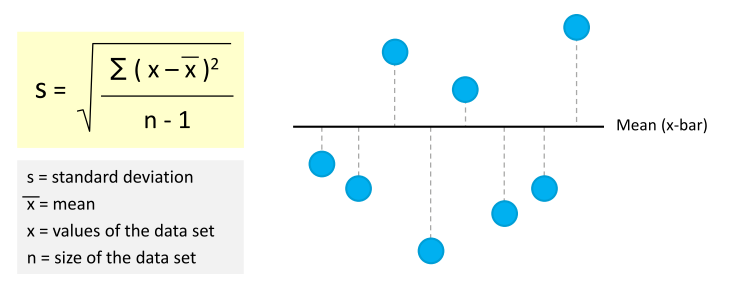
\includegraphics[width=0.5\linewidth,keepaspectratio]{da16}
\end{center}

\begin{lstlisting}
def variance(datalist):
	:
	return v

def std_dev(datalist):
	:
	return s

lst = [9,3,7,2,7,10,23,44,12,42,19,11,22,5,3,4,3,21,3]
result1 = variance(lst)
result2 = std_dev(lst)
print("Variance {}, Std Dev {}".format(result1,result2))
\end{lstlisting}
\end{frame}

%%%%%%%%%%%%%%%%%%%%%%%%%%%%%%%%%%%%%%%%%%%%%%%%%%%%%%%%%%
\begin{frame}[fragile]\frametitle{Variance, Standard Deviation}
\begin{lstlisting}
def de_mean(x):
	"""translate x by subtracting its mean"""
	x_bar = mean(x)
	return	[x_i - x_bar for x_i in x]

def sum_of_squares(diffs):
	sum_of_squares = 0
	for df in diffs:
          sum_of_squares += (df) ** 2
     return sum_of_squares

def variance(x):
	"""assumes x has at	least two elements"""
	n = len(x)
	deviations = de_mean(x)
	return	sum_of_squares(deviations) / (n - 1)
 
def std_dev(anotherlist):
	std_dev = variance(anotherlist) ** 0.5
	return std_dev
\end{lstlisting}
Variance 158.36257309941527, Std Dev 12.584219208970229
\end{frame}


%%%%%%%%%%%%%%%%%%%%%%%%%%%%%%%%%%%%%%%%%%%%%%%%%%%%%%%%%%%%%%%%%%%%%%%%
\begin{frame}[fragile]\frametitle{Covariance}
Implement covariance, the paired analogue of variance.
The variance measures how a single variable deviates from its mean, covariance measures how two variables vary in tandem from their means.
\begin{center}
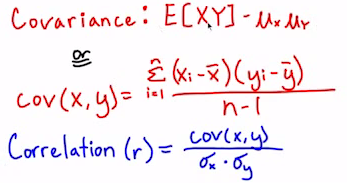
\includegraphics[width=0.5\linewidth,keepaspectratio]{corrcov}
\end{center}
\begin{lstlisting}
x = [2, 3, 0, 1, 3]
y = [ 2, 1, 0, 1, 2]
result1 = covariance(x,y)
result2 = correlation(x,y)print("CoVariance {}, Correlation {}".format(result1,result2))
\end{lstlisting}
\end{frame}

%%%%%%%%%%%%%%%%%%%%%%%%%%%%%%%%%%%%%%%%%%%%%%%%%%%%%%%%%%
\begin{frame}[fragile]\frametitle{Covariance}
Covariance is like a dot product and tell how two quantities (centered, meaning subtracted by Mean) are together/similar.
\begin{lstlisting}
def elemwise_multi(v, w):
    """v_1 * w_1 + ... + v_n * w_n"""
    return sum(v_i * w_i for v_i, w_i in zip(v, w))

def covariance(x, y):
	n = len(x)
	return	elemwise_multi(de_mean(x), de_mean(y)) / (n - 1)

\end{lstlisting}
CoVariance 0.8
\end{frame}

%%%%%%%%%%%%%%%%%%%%%%%%%%%%%%%%%%%%%%%%%%%%%%%%%%%%%%%%%%
\begin{frame}[fragile]\frametitle{Correlation}
Covariance is like a dot product normalized by standard deviation.
\begin{lstlisting}
def correlation(x, y):
	stdev_x = std_dev(x)
  	stdev_y = std_dev(y)
	if stdev_x > 0 and stdev_y > 0:
		return	covariance(x, y) / stdev_x / stdev_y
	else:
		return	0 # if	no variation, correlation is zero
\end{lstlisting}
Correlation 0.7333587976225691
\end{frame}


%%%%%%%%%%%%%%%%%%%%%%%%%%%%%%%%%%%%%%%%%%%%%%%%%%%%%%%%%%%%%%%%%%%%%%%%
\begin{frame}[fragile]\frametitle{Normal Distribution}
The classic bell curve-shaped distribution and is completely determined by two parameters: its mean (mu) and its standard deviation	 (sigma).
\begin{center}
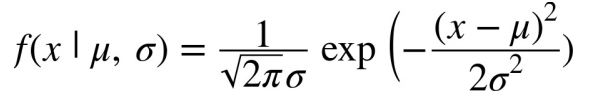
\includegraphics[width=\linewidth,keepaspectratio]{normdisteq}
\end{center}
Implement. 

Use \lstinline|math.sqrt| and \lstinline|math.pi| as well as \lstinline|matplotlib.pyplot| for plotting
\begin{lstlisting}
def normal_pdf(x, mu=0, sigma=1):
	:
	return v
\end{lstlisting}
\end{frame}

%%%%%%%%%%%%%%%%%%%%%%%%%%%%%%%%%%%%%%%%%%%%%%%%%%%%%%%%%%%%%%%%%%%%%%%%
\begin{frame}[fragile]\frametitle{Normal Distribution}
Data and plotting routine
\begin{lstlisting}
xs=[x	/10.0 for x in range(-50, 50)]

plt.plot(xs,[normal_pdf(x,sigma=1) for x in xs],'-')
plt.plot(xs,[normal_pdf(x,sigma=2) for x in xs],'--')
plt.plot(xs,[normal_pdf(x,sigma=0.5) for x in xs],':')
plt.plot(xs,[normal_pdf(x,mu=-1) for x in xs],'-')
plt.legend()
plt.title("Normal pdfs")
plt.show()
\end{lstlisting}
\end{frame}

%%%%%%%%%%%%%%%%%%%%%%%%%%%%%%%%%%%%%%%%%%%%%%%%%%%%%%%%%%%%%%%%%%%%%%%%
\begin{frame}[fragile]\frametitle{Normal Distribution}
\begin{lstlisting}
import math
import matplotlib.pyplot as plt
def normal_pdf(x, mu=0, sigma=1):
	sqrt_two_pi = math.sqrt(2*math.pi)
	return	(math.exp(-(x-mu)**2/2/sigma**2) / (sqrt_two_pi* sigma))
\end{lstlisting}
\end{frame}

%%%%%%%%%%%%%%%%%%%%%%%%%%%%%%%%%%%%%%%%%%%%%%%%%%%%%%%%%%%%%%%%%%%%%%%%
\begin{frame}[fragile]\frametitle{Normal Distribution}
\begin{center}
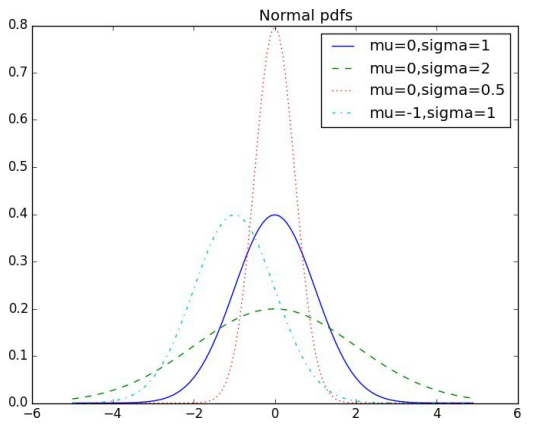
\includegraphics[width=0.8\linewidth,keepaspectratio]{normdistplot}
\end{center}
\end{frame}
